\section{Data Preprocessing: The REPLICA Pipeline}
\label{sec:data_preprocessing}

As established in Section~\ref{sec:background_eventcamera}, an event camera outputs a sparse, asynchronous stream of events $e = (x, y, t, p)$, where $(x, y)$ are the spatial coordinates, $t$ is the microsecond timestep, and $p \in \{-1, 1\}$ is the polarity indicating an increase or decrease in brightness.
The \texttt{REPLICA} preprocessing pipeline takes the raw \gls{etram} data at $1280 \times 720$ spatial resolution and converts it into the dense, structured tensor format required by the \gls{snn} and \gls{cnn} backbones.

\subsection{Raw Event Ingestion \& Windowing}

The \texttt{REPLICA} pipeline begins by reading the raw h5 event files $(x, y, t, p)$ and the partnering npy files containing the bounding box annotations from the \gls{etram} dataset.
Once both files have been parsed, the first step taken is to apply a $100 ms$ sliding window across the entire duration of the event file. 
``Windowing`` is the process of slicing the continous event stream into chunks that represent a single instance of time for the model, thereby anchoring the asynchronous event stream into discrete, structured training instances. 

To maximize training efficiency and ensure a high signal-to-noise ratio in the training distribution, the \texttt{REPLICA} pipeline adopts a Box-Central sampling strategy rather than more conventional uniform temporal partitioning, where training windows were anchored deterministically around the centroids of
existing ground truth annotations. This approach ensures that 100\% of the training voxels contain informative structural targets, mitigating the prevalence of 'empty-scene' noise and providing the SNN with consistent temporal evidence to drive membrane potential
accumulation prior to the target timestamp.

In this project, the time window $\Delta T = 100\text{ms}$ was chosen to align with the temporal persistency of the human visual system of roughly $100\text{ms}$ \cite{deodato2024continuous};
just as the human eye integrates luminance changes over approximately one frame of perception, the \gls{snn} also integrates the asynchronous event stream over the same duration before producing a detection output.

The practical consequence of this choice is two-fold. 
First, a $100\text{ms}$ window is long enough to guarantee a minimum event density sufficient for the \gls{lif} neurons 
in the stem layer to accumulate membrane potential and produce meaningful spike trains 
across all $T = 10$ temporal bins. 
Second, specific to the context of vehicle detection, it is short enough that a vehicle travelling at highway speed (e.g., $120\text{ km/h} \approx 33\text{ ms}^{-1}$) displaces by 
only $3.3\text{m}$ within the window, ensuring that the bounding box annotation 
assigned to the window remains spatially valid and does not introduce label noise through excessive object displacement.

In combination with the Box-Central sampling approach, the pipeline applies a density filter prior to voxelization to enforce a minimum quality threshold in valid samples. 
For each $100\text{ms}$ window, the total number of raw $(x, y, t, p)$ events is counted: windows containing fewer than 
\texttt{min\_events} $= 500$ events are discarded, while those meeting or exceeding this threshold proceed to voxelization as valid training samples.
This filter is a structural necessity for \gls{snn} training stability:

\begin{itemize}

    \item \textbf{Prevention of dead neurons:}
    \glspl{snn} are metabolic models: they require energy (spikes) to learn. 
    Training on near-empty windows rewards the optimiser for suppressing all firing, 
    driving synaptic weights so low that even high-density frames containing real vehicles 
    fail to trigger a spike response \cite{eshraghian2021training}.

    \item \textbf{\gls{frr} stability:}
    The \gls{frr} loss penalises deviation from a target firing rate of $20\%$ 
    \cite{deng2021comprehensive, yan2022backpropagation}. Presenting near-empty 
    inputs forces the regularisation term to dominate the total loss, as it 
    attempts to generate spikes in the absence of any meaningful input signal.

    \item \textbf{Gradient quality:}
    A forward pass producing no spikes yields a zero surrogate gradient 
    \cite{neftci2019surrogate}. Training on empty windows is therefore 
    mathematically degenerate since no weight update occurs, so \gls{hpc} cycles 
    are consumed without any learning signal.

    \item \textbf{Background activity suppression:}
    Event cameras produce a baseline level of Background Activity (BA) noise 
    from transistor mismatch and thermal effects \cite{gallego2020event}. 
    A window containing less than 500 events is statistically likely to consist 
    almost entirely of noise; the \texttt{min\_events} threshold therefore 
    functions as a signal intensity floor, directing the model's attention 
    exclusively towards windows in which a meaningful scene change has occurred.

\end{itemize}

\subsection{Signal Conditioning}

THe first step of the \texttt{REPLICA} pipeline is to apply a series of signal conditioning operations to the raw event data to improve the \gls{snr}, which yields several benefits:

\begin{itemize}
    \begin{sloppypar}
    \item \textbf{Prevention of \gls{lif} neuron saturation:} 
    \end{sloppypar}
    Without input conditioning, high-magnitude or noisy voxel values can drive every neuron in the initial stem layer to fire continuously and flood the network with uninformative spikes. 
    By normalising the voxel tensor to the range $[0, 1]$, the input magnitude is constrained such that only neurons encoding genuine structural features,such as vehicle edges 
    and motion boundaries, exceed their firing threshold, preserving the sparsity and selectivity of the deeper backbone stages \cite{eshraghian2021training}.

    \item \textbf{Improved objectness discrimination:}
    Background artifacts inherent to \gls{hd} event cameras, such as flickering illumination and sensor noise, generate erraneous event clusters that appear similar to small objects. 
    By rejecting these low-activity events during the \gls{baf} denoising step, the network is not required to expend representational capacity on learning to suppress noise, 
    and can instead focus on learning the geometric structure of real vehicles \cite{eshraghian2021training, Roy2019SpikeBasedMI}.

    \item \textbf{Reduced synaptic operations and neuromorphic energy efficiency:}
    Since \glspl{snn} consume energy only upon spike emission, every erraneous background event that is suppressed during preprocessing directly reduces the number of \glspl{sop} at inference time. 
    This establishes a direct link between preprocessing quality and the power efficiency of the architecture when deployed on neuromorphic hardware \cite{Roy2019SpikeBasedMI}.
\end{itemize}

The Signal Conditioning segment of the \texttt{REPLICA} pipeline was lifted directly from the original \gls{etram} study, since it was designed specifically to suit the characteristics of the dataset \cite{Verma_2024_CVPR}.

\subsection{Spatiotemporal Voxelization}

To make the asynchronous event data compatible with neural network layers, a Voxelization process is performed to transform the continuous stream into a structured tensor. This process consists of three core operations:

\begin{itemize}
    \item \textbf{Temporal Binning:} The total duration of an event sample (e.g., a 100ms window) is divided into 10 discrete time bins ($T=10$).
    \item \textbf{Polarity Splitting:} Events are separated into two distinct channels based on their polarity ($C=2$), representing positive and negative brightness changes.
    \item \textbf{Event Accumulation (Histogramming):} Within each discrete temporal bin and polarity channel, the individual asynchronous events are aggregated at their respective spatial coordinates $(x,y)$. Specifically, the value of each ``pixel'' in the resulting spatial grid becomes the total count of events (of that specific polarity) that occurred at that exact location during that fraction of time. This process effectively converts the sparse, continuous point-cloud of events into a sequence of dense 2D frames---or event histograms---which standard convolutional and spiking layers can natively process.
\end{itemize}

This accumulation process preserves the temporal distribution of the events while generating a dense 4D spatiotemporal tensor of shape $[10, 2, 720, 1280]$ (representing Time $\times$ Channels $\times$ Height $\times$ Width).

\subsection{Downsampling \& Normalization}
Following spatiotemporal voxelization, the voxelized data undergoes a dual-phase refinement consisting of spatial downsampling and amplitude normalization. 
This is the final polishing step of the pipeline, transforming the high-resolution event counts into a stabilized, low-memory format that the neural backbones can process efficiently.

\subsubsection{Spatial Downsampling (16-fold Data Reduction)}
The generated high-definition voxel grid ($1280 \times 720$) is subjected to a $4 \times 4$ Max-Pooling operation, reducing the spatial resolution to $320 \times 180$. 
This 16-fold reduction in data volume is critical for managing the high-dimensional state-space of the \gls{snn} backbone. 
Because \glspl{snn} must store neuron membrane potentials across time, an HD model would require massive amounts of GPU memory. 
By aggressively reducing the spatial dimensions, we ensure the backbone scalability, making it computationally feasible to train the deep 4-block architecture over extended epochs.

Furthermore, utilizing Max-Pooling (as opposed to Average-Pooling) acts as a feature preserver: it retains the strongest event signal within each $4 \times 4$ area, helping the network maintain the crisp, high-contrast edges of the vehicles even at a lower resolution.

It should be noted that the downsampling factor $ds = 4$ was heavily influenced by the \gls{hpc} cluster's GPU memory constraints; without using $ds = 4$,
the data would not fit into the GPU memory, or would require a batch size of 1, making training infeasible within the time constraints of this project.

\subsubsection{Max-Normalization (Input Calibration)}

Subsequently, max-normalization is performed to scale the raw event accumulation counts into a continuous $[0, 1]$ interval,
by dividing every pixel in the temporal volume by the single highest event count found within that 10-bin voxel.

This normalization serves as a fundamental safeguard against neural saturation. 
\gls{lif} nodes have fixed firing thresholds (in this architecture, $V_{th}=0.2$) - if a raw, unscaled event count of 50 were fed into the network, the first-layer neurons would fire instantaneously and repeatedly, effectively ``screaming'' and drowning out all other spatiotemporal information. 
By enforcing input calibration, we ensure that the input magnitudes are calibrated relative to the \gls{lif} thresholds, facilitating stable surrogate gradient propagation during the 150-epoch training cycle.

\subsection{Multi-Object Label Alignment}
\label{subsec:multi_object_alignment}

The final stage of the pipeline implements a Multi-Object Label Alignment strategy, which is fundamental to the architecture's multi-object detection capabilities. 
This stage transforms individual, asynchronous bounding box annotations into structured, scale-independent target tensors suitable for the network's multi-box regression head.

\subsubsection{Timestamp-Based Grouping (Unified Scene Representation)}
Instead of creating isolated training samples for every individual vehicle, the pipeline parses the ground truth annotations and groups all vehicles that exist at the exact same microsecond ($t$). 
This process merges individual detections into a Unified Scene Representation, 
which is crucial because it eliminates ``label noise''; presenting the network with identical visual input but different single-car targets across multiple samples would force the model to average its predictions, resulting in blurry, low-confidence bounding boxes with poor \gls{iou} scores.

\subsubsection{Fixed-Capacity Padding}
Deep learning models inherently require consistent tensor dimensions for batched training. 
To accommodate scenes with varying numbers of vehicles, we enforce a Fixed-Capacity Interface of exactly 5 bounding boxes per frame. 
If a scene contains 2 vehicles, the remaining 3 slots are populated with ``empty'' zero-padded boxes. 
If a frame contains no vehicles, 5 empty boxes are provided. This ensures every target label is a consistent $[5, 5]$ tensor. 
The limit of 5 boxes was empirically selected based on an analysis of the \gls{etram} validation set, where the vast majority of frames contain 3 or fewer vehicles, making 5 a safe upper bound for this specific traffic monitoring environment.

\subsubsection{Binary Masking}
To enable the network to distinguish between genuine vehicle targets and zero-padded instances, the tensor utilizes a Binary Masking dimension. 
For every box, the target tensor stores five values: $[Center_X, Center_Y, Width, Height, Mask]$.
\begin{itemize}
    \item For a real object, the mask value is set to $1.0$.
    \item For a padded or empty box, the mask value is set to $0.0$.
\end{itemize}
This mask acts as the objectness confidence target. 
It is utilized by the Multi-Box Loss function to selectively apply coordinate gradients only to valid targets, while simultaneously regularizing the model's confidence head to output $0.0$ for empty regions.

\subsubsection{Normalization to Sensor Space}
Finally, all spatial parameters (center coordinates, width, and height) are originally provided in raw pixel values (e.g., $x=842$). 
These are normalized by dividing by the raw sensor width ($1280$) and height ($720$), scaling all coordinates into the continuous range $[0.0, 1.0]$. 
This provides a Scale-Independent Signal, ensuring the regression head can learn the underlying geometry robustly, regardless of the spatial downsampling factors applied earlier in the pipeline.

\subsection{Chunking for High-Throughput I/O}
\label{subsec:chunking}

Training the model for 150 epochs is only feasible if the \texttt{REPLICA} pipeline is executed once rather than on every epoch.
A naive dataloader would stream the raw h5 and npy files in whatever segment fits in memory and re-run the full pipeline (signal conditioning, voxelisation, downsampling, label alignment) on each pass, multiplying the preprocessing cost 150-fold and starving the \gls{gpu} while the CPU works through every voxelisation and denoising call.

The chunking strategy moves the preprocessing out of the training loop entirely.
The \texttt{REPLICA} pipeline is executed once, offline, and the resulting spatiotemporal voxels and aligned label tensors are serialised to disk as contiguous 250-sample chunks (compressed \texttt{.pt}), indexed by a global \texttt{manifest.json} byte-offset map.
During training, the dataloader reads these precomputed chunks directly into VRAM, so the 150 epochs execute against structured tensors rather than raw events.

\subsubsection{LRU Caching in \texttt{VoxelDiskDataset}}

To further amortise disk I/O, the custom \texttt{VoxelDiskDataset} wraps the chunk layout with a \gls{lru} memory cache sized to hold the full 40-chunk dataset in the node's 120\,GB RAM.
During Epoch~1, chunks are read from NFS into memory as the dataloader encounters them, populating the cache in full.
Every subsequent epoch is then served entirely from RAM, so the training loop never touches disk after Epoch~1.
The \gls{lru} eviction policy is a safety net for cache-smaller-than-dataset configurations: the least-recently-used chunk is evicted to make room for the next load, ensuring the hot data is always ready for the \gls{gpu}.

The combined effect of offline precomputation, chunked serialisation, and in-memory caching reduces the 150-epoch wall time from a projected multi-day run to approximately six hours at $\sim$160\,ms/iter.

\subsection{REPLICA Pipeline: Visualized}

Figure \ref{fig:preprocessing_pipeline} details the order of which the aformentioned preprocessing steps are applied to the raw event data.

\begin{figure}[htbp]
    \centering
    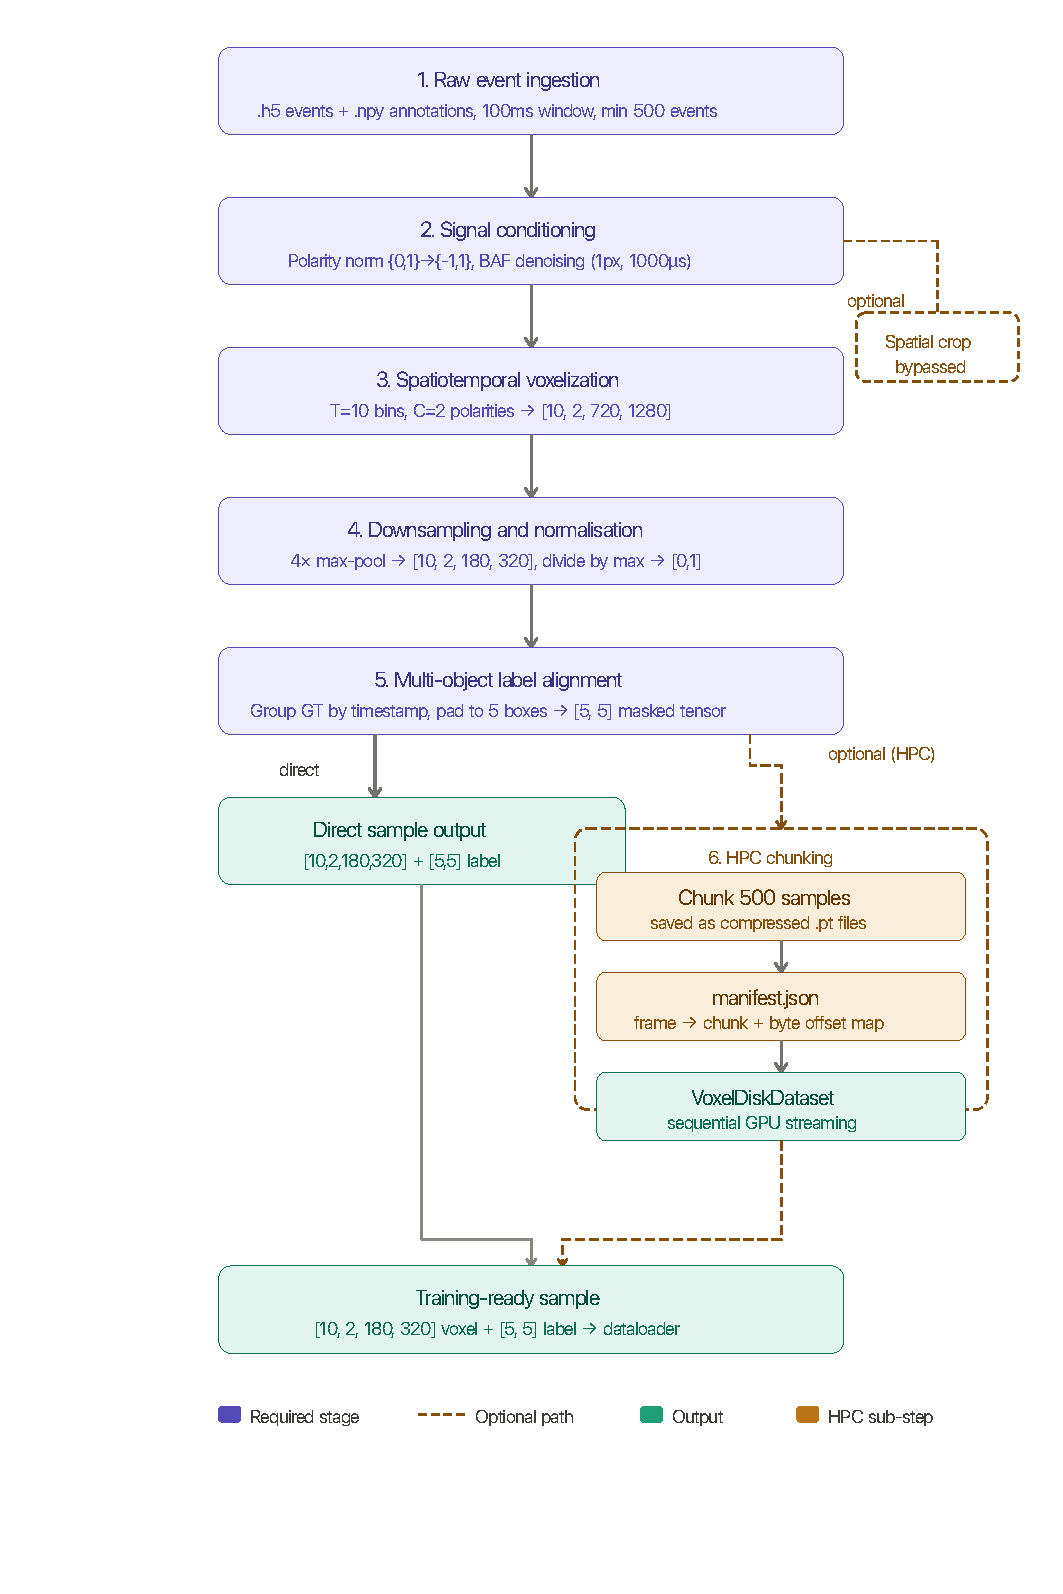
\includegraphics[width=0.8\textwidth]{chapter_3/figures/preprocessing_pipeline.pdf}
    \caption{Overview of the spatiotemporal preprocessing pipeline applied to the ETraM dataset.
    Raw events are voxelized into a 4D tensor, spatially downsampled, and aligned with
    multi-object ground truth labels to produce a final sample of shape \texttt{[10, 2, 180, 320]}
    with a corresponding label tensor of shape \texttt{[5, 5]}.}
    \label{fig:preprocessing_pipeline}
\end{figure}

\clearpage